\chapter{Theory}
This section addresses necessary theory needed to understand the project.

\section{Naive Bayes}
Naive Bayes is a generative model that models multinomial data, and is consequently suitable for multi-class classification problems. When presented with a new data point $x$ it assigns to it the class $C_k$ such that $C_k$ maximises the posterior class probabilities under the assumption that the observed data $X$ is independently drawn, which gives
\begin{equation}
    P(C_k | X) \propto P(X | C)P(C) = \prod_{i}^{N}P(x_{i}|C_{k})P(C_{k}), 
\end{equation}
that can be computed easily. However, should a previously unseen word
appear the conditional probability of the word would be
$P(x_i|C_k)=0$. This is typically solved by assuming $C_{k} \sim
Dirichlet(\alpha)$ for a small $\alpha$, which by
multinomial-dirichlet conjugacy gives the maximum a posteriori esimate
\begin{equation}
  E[C_{k} | X] = \frac{x_{k}+ \alpha_{k}}{N + \sum_{j=1}^{K}\alpha_{j}},
\end{equation}
that does not suffer the same problem, since the numerator is never $0$ even for observed counts $x_{k} = 0$.

\section{FastText Word Embeddings}
Like the word2vec model, which learns vector representations of
words~\cite{Mikolov2013Jan}, FastText is also a technique for vector
embedding words. However, FastText does not learn a vector for each
word but for each charecter $n$-gram in each
word~\cite{Bojanowski2016Jul}. It also includes special start and end
symbols <, and >, to be able to distinguish prefixes and suffixes, and
the whole word as a special sequence. For example, the word
\textit{horse} induce the character 3-grams <ho, hor, ors, rse, se>
and the special sequence <horse>. In practice, the set of all
$n$-grams $G_w$ for word $w$ are computed for $n = 3, 4, 5, 6$. The embedding of
$w$ is then given by the sum of the vector representations of all
$g \in G_w$.

\section{Recurrent Neural Networks}
Recurrent Neural Networks (RNNs) are a flavour of Artificial Neural Networks (ANNs) designed to work with sequential data~\cite{goodfellow2016deep}. While an ANN can be presented with sequential data as well, it lacks the capability of preserving a context throughout it. This is solved by RNNs by introducing dependencies on previous sequential steps through additional connections.
\begin{figure}[H]
  \centering
  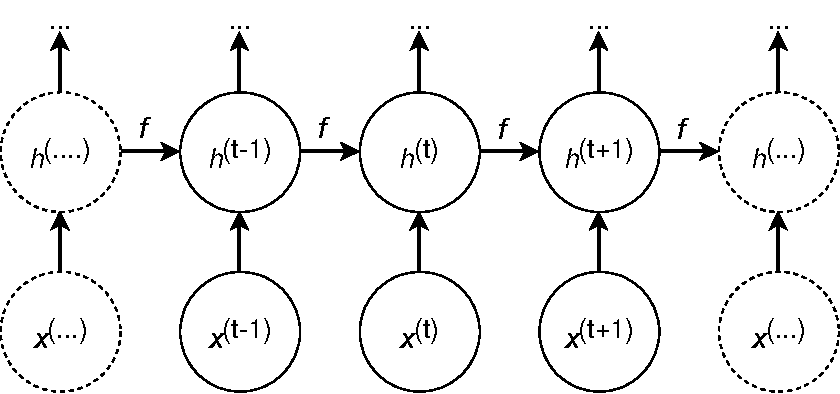
\includegraphics[width=0.8\textwidth]{graphics/rnn-2}
  \caption{An illustration of an RNN for input sequence $x$, where $h$ is the hidden unit activation functions and $f$ a function describing the relationship between two concurrent states~\cite{goodfellow2016deep}.}\label{fig:rnn}
\end{figure}
An illustration of an RNN can be seen in Figure~\ref{fig:rnn} which
shows the context-preserving connections between the hidden nodes
$h^{(t)}$. There are many ways to structure RNNs depending on the
problem at hand, but other structures are out of scope for this project.

Training of RNNs is done using the \textit{backpropagation} algorithm, which is an efficient way to perform gradient descent optimisation of the networks weights. However, in the case of long-term dependencies the gradients tend to become vanishingly small (or in some rare cases tend towards infinity) which hinders training. One solution to this problem is to use so called \textit{gated RNNs}; in particular Long Short-Term Memory Networks (LSTMs).

\subsection{Long Short-Term Memory Networks}
LSTMs are RNNs with a more complicated cell structure for the hidden units, which have shown to much better capture long-term dependencies than the simpler structure of standard hidden units~\cite{hochreiter1997long}. They work by containing an internal state which is regulated by the input.

\begin{figure}[H]
  \centering
  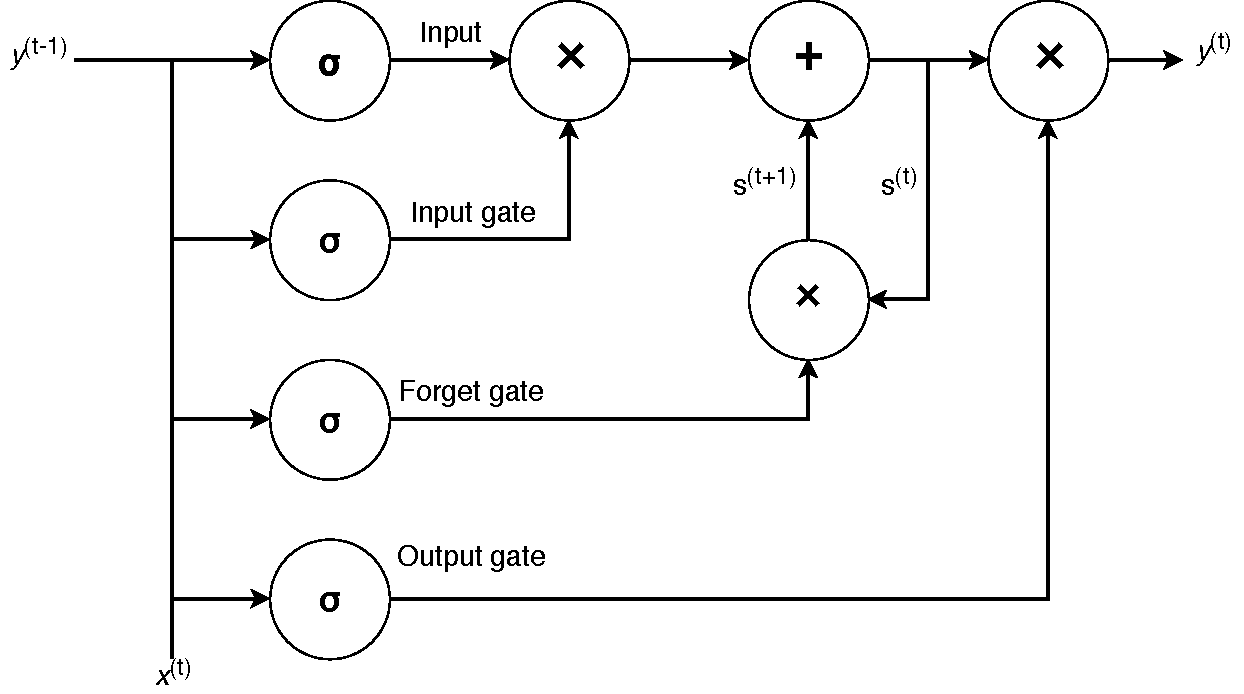
\includegraphics[width=0.8\textwidth]{graphics/lstm-cell}
  \caption{An illustration of an LSTM cell where $x$ is input, $y$ output and $s$ cell state for a specific time point. $\sigma$ indicates a linear combination of inputs passed through the sigmoid function. }\label{fig:lstm-cell}
\end{figure}
As can be seen in Figure~\ref{fig:lstm-cell} an LSTM propagates both the previous output $y^{(t-1)}$ and the previous state $s^{(t-1)}$ to the next cell. This comes at the cost of several more weights that need to be optimised during training, but is a key component for their performance.